\documentclass[a4paper,11pt]{ltjsarticle}
% 数式
\usepackage{amsmath,amsfonts}
\usepackage{bm}
% 画像
\usepackage{graphicx}
\usepackage{circuitikz}
\usepackage{amsmath,amssymb}
\usepackage{siunitx}
\usepackage{float}
\usepackage{tikz}
\usepackage{askmaps}
\usepackage{multirow}
\usepackage{bigstrut}
\usepackage{slashbox}
\usepackage{rotating}
\usepackage{listings}
% 数式
\usepackage{physics}
\usepackage{mathtools}
% 画像
\usepackage{subcaption}
% 表
\usepackage{makecell}
% その他
\usepackage{url}
\usepackage{ascmac}
\usepackage{cases}
\usepackage{here}
\usepackage{upgreek}
% 日本語対応
\usepackage{luatexja}
\usepackage{luatexja-fontspec}

\AtBeginDocument{\RenewCommandCopy\qty\SI}


\definecolor{commentgreen}{RGB}{0,200,0}
\definecolor{eminence}{RGB}{120,80,250}
\definecolor{weborange}{RGB}{255,165,0}
\definecolor{frenchplum}{RGB}{10,150,200}
\definecolor{commentgreen}{RGB}{0,200,0}
\definecolor{eminence}{RGB}{120,80,250}
\definecolor{weborange}{RGB}{255,165,0}
\definecolor{frenchplum}{RGB}{10,150,200}

\lstset{
        language = {C},
        basicstyle = \ttfamily\small,
        keywordstyle=\color{eminence}\ttfamily\bfseries,
        commentstyle=\color{commentgreen}\textit,
    identifierstyle=\color{black}\ttfamily,
        xleftmargin=.35in,
        frame=lines,
    showstringspaces=false,
        numbers=left,
        stepnumber = 1,
        breaklines=true,
        numberstyle = \ttfamily\normalsize,
    tabsize=4,  
        emph={int, int8_t, int16_t, int32_t, int64_t, uint8_t, uint16_t, uint32_t, uint64_t, char, double, float, unsigned, void, bool},
        emphstyle={\color{blue}}, 
        morekeywords={>, <, ., ;, +, -, *, /, !, =, ~},
        breakindent = 10pt, 
        framexleftmargin=10mm, 
        columns=fixed,
        basewidth=0.5em,
        }

% 特定のスタイル設定
\lstdefinestyle{customtxt}{
  basicstyle=\ttfamily\footnotesize,
  backgroundcolor=\color{lightgray},
  frame=single,
  breaklines=true,
  columns=fullflexible,
  showspaces=false,
  showstringspaces=false,
  showtabs=false,
  tabsize=4,
}

\newcommand{\fig}[4]{
    \begin{figure}[htbp]
      \centering
      \includegraphics{./images/#1}
      \caption{#2}
      \label{fig:#3}
    \end{figure}
  }
\begin{document}
\begin{flushright}
    22060 古城 隆人\\
\end{flushright}
\section{はじめに}
数値解析における代表的な方程式の解法として,
二分法,はさみうち法,ニュートンラプソン法がある.
これらの方法は,それぞれ収束性や特性が異なるため,実際に計算を行い比較することで理解を深めることができる.
\subsection{二分法}
二分法では,関数が連続であり,初期値の間に必ず解があることがわかる場合に使用することが出来る.
初期値の間を半分に分割し,半分の値の符号を判断することにより,どちらに買いが存在するかを判定し,半分の値をまた初期値として計算を行っていく方法である.
この方法では収束に時間がかかるが,必ず解に収束するという特徴がある.\cite{nibunhou}
\subsection{はさみうち法}
はさみうち法では,関数が連続であり,初期値の間に必ず解があることがわかる場合に使用することが出来る.
初期値a,bに直線を引き,その直線とx=0が交わる点をcとして,点cのx座標における求めたい関数の値を求める.
その点の符号から,解の存在する場所を判定し,また直線を引くを繰り返す.二分法よりも収束が速い場合もあるが,必ずしも速いとは限らない.\cite{hasamiutihou}
\subsection{ニュートンラプソン法}
ニュートンラプソン法では,関数の微分が求められる場合に使用することが出来る.
初期値における関数の接線を求め,その接線とx=0が交わる点を次の初期値として計算を行っていく方法である.
この方法では収束が非常に速いが,初期値によっては発散する場合もある.\cite{newtonrapsonhou}
\section{実験方法}
Excelを用いて,二分法,はさみうち法,ニュートンラプソン法をステップごとにもとめ,グラフにより収束性や特性を確認する.
そのために,初期値を変更した二回の実験を行う.また,使用する式は式\eqref{eq:func}とする.
\begin{equation}
    f(x) = \cosh(x)\cos(x) + 1
    \label{eq:func}
\end{equation}
実験1の初期値を表\ref{tab:init1}に示す.
実験2の初期値を表\ref{tab:init2}に示す.
\begin{table}[H]
    \centering
    \caption{各方式の初期条件}
    \begin{tabular}{|c|c|c|}
        \hline
        方式         & 初期値1 & 初期値2 \\ \hline
        二分法        & 0    & 1    \\ \hline
        はさみうち法     & 0    & 1    \\ \hline
        ニュートンラプソン法 & 1    & -    \\ \hline
    \end{tabular}
    \label{tab:init1}
\end{table}
\begin{table}[H]
    \centering
    \caption{各方式の初期条件}
    \begin{tabular}{|c|c|c|}
        \hline
        方式         & 初期値1 & 初期値2 \\ \hline
        二分法        & 0    & 2    \\ \hline
        はさみうち法     & 0    & 2    \\ \hline
        ニュートンラプソン法 & 2    & -    \\ \hline
    \end{tabular}
    \label{tab:init2}
\end{table}


\section{実験結果}
実験1の結果を図\ref{fig:result1},実験2の結果を図\ref{fig:result2}に示す.
\begin{figure}[H]
    \centering
    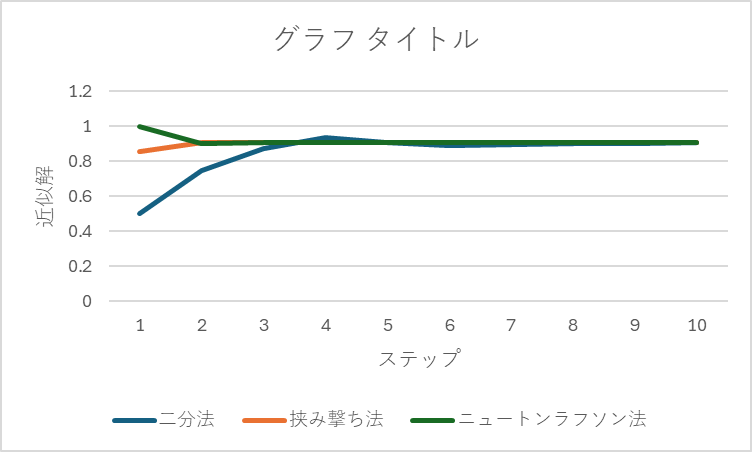
\includegraphics[width=12cm]{./images/result1.png}
    \caption{各方式の結果}
    \label{fig:result1}
\end{figure}
\begin{figure}[H]
    \centering
    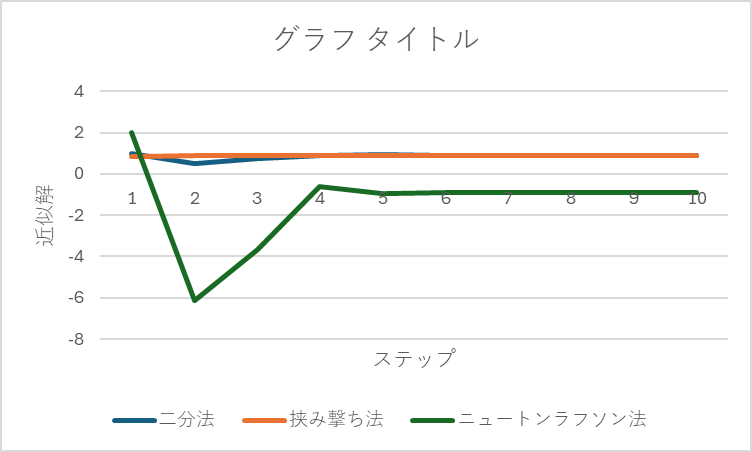
\includegraphics[width=12cm]{./images/result2.png}
    \caption{各方式の結果}
    \label{fig:result2}
\end{figure}


\section{考察}
実験結果より,各方式の収束性や特性について以下のことがわかった.
\begin{itemize}
    \item 二分法は,必ず解に収束するが,収束に時間がかかる.
    \item はさみうち法は,二分法よりも早く収束した.
    \item 二分法では想定解に近づいても値がオーバーすることがわかった.
    \item ニュートンラプソン法は,非常に速く収束したが,実験2では値が発散し,想定解と大きく外れる解に収束した.
    \item 各方式の収束性は,初期値によっても変化することがわかった.
\end{itemize}
Kono結果より,今回の方程式では挟み撃ち法を用いれば,大体の解においては収束が安定して早く求められるのではないのかなと思った.

\begin{thebibliography}{9}
    \bibitem{nibunhou} 伊津野和行・酒井久和, Excelではじめる数値計算解析, 森北出版株式会社, p.66.,2024.
    \bibitem{hasamiutihou} 伊津野和行・酒井久和, Excelではじめる数値計算解析, 森北出版株式会社, p.68.,2024.
    \bibitem{newtonrapsonhou} 伊津野和行・酒井久和, Excelではじめる数値計算解析, 森北出版株式会社, p.64.,2024.
\end{thebibliography}

\end{document}